\documentclass[conference]{IEEEtran}
\IEEEoverridecommandlockouts
% The preceding line is only needed to identify funding in the first footnote. If that is unneeded, please comment it out.
\usepackage{cite}
\usepackage{amsmath,amssymb,amsfonts}
\usepackage{algorithmic}
\usepackage{graphicx}
\usepackage{textcomp}
\usepackage[export]{adjustbox}
\usepackage{xcolor}
\def\BibTeX{{\rm B\kern-.05em{\sc i\kern-.025em b}\kern-.08em
    T\kern-.1667em\lower.7ex\hbox{E}\kern-.125emX}}
\begin{document}

\title{Predicting Retail Gasoline Prices using Long Short-Term Memory Recurrent Neural Networks\\
}

\author{\IEEEauthorblockN{Hector E. Lopez}
\IEEEauthorblockA{\textit{College of Engineering and Computer Science} \\
\textit{University Of Texas Rio Grande Valley}\\
Edinburg, Texas, United States of America \\
hector.e.lopez01@utrgv.edu}
\and
\IEEEauthorblockN{Victor J. Martinez}
\IEEEauthorblockA{\textit{College of Engineering and Computer Science} \\
\textit{University of Texas Rio Grande Valley}\\
Edinburg, Texas, United States of America \\
victor.martinez05@utrgv.edu}
}

\maketitle

\begin{abstract}
This document details a machine learning implementation that predicts the average retail gas station prices for the state of Texas. It further explains the process and work flow that went into data gathering and processing. Any Challenges we faced, and the results of the implementation. Concluding with future plans for the project.
\end{abstract}

\begin{IEEEkeywords}
data, WTI, LSTM, csv, method, sklearn, keras
\end{IEEEkeywords}

\section{Introduction}

Gas station prices fluctuate throughout the year, with the crude oil barrel prices arguably being the most influential factor affecting these prices. Seasons throughout the year also influence the retail gas prices, such as summer, when most people take vacations. Our goal for this project was to be able to accurately predict retail gas prices based on the season and crude oil barrel prices. This would allow a person to judge whether to fill up their vehicle or wait a couple days if the gas prices are projected to fall. Through our process of data gathering, we saw gas station price swings vary as much as 70 cents in a matter of a weeks. More modest swings were about 30 cents however. With full sized pickup trucks having gas tanks in the 20-40 gallon range, and the most economic ones coming around 20 miles per gallon[1], a person driving a modest 10,000 miles a year could save roughly \$150 a year, using the previously mentioned 30 cent swings. So, as you can imagine, being able to implement this in a mobile phone application would be highly beneficial to people on a very tight budget, making it our main motivation. 

\section{Data}

For the purposes of the project, we knew we needed some type of crude oil price. We discovered WTI crude oil barrel prices, and how that was used for Texas gas stations. The decision to include WTI was made because of its direct relationship with gas station prices, and the possibility that the window between the change of crude oil and gas station prices would be enough to help the model with accuracy. Initially, we scraped hourly prices from twelve local gas stations in the Edinburg, Tx area, along with hourly WTI prices for four weeks. Ultimately, however, we didn’t have enough data for an accurate model. On top of that, the hourly gas station prices were dependent on user input, leading to gas station prices not being updated for days at a time, or not having a price at all at some points, tainting our dataset. Our final data we settled on was weekly Texas-wide average gas station retail prices, and weekly WTI barrel prices, from June 05, 2000 to November 11, 2019[2][3]. In the end, our data was in a csv file with the date, WTI price, and Texas avg gas price. Our model implementation also added two additional attributes, month, and day, so our network could hopefully learn seasons. 

\begin{figure}[htbp]
\includegraphics[width=.99\linewidth]{csv.png}
\caption{Base data.}
\label{fig}
\end{figure}

\begin{figure}[htbp]
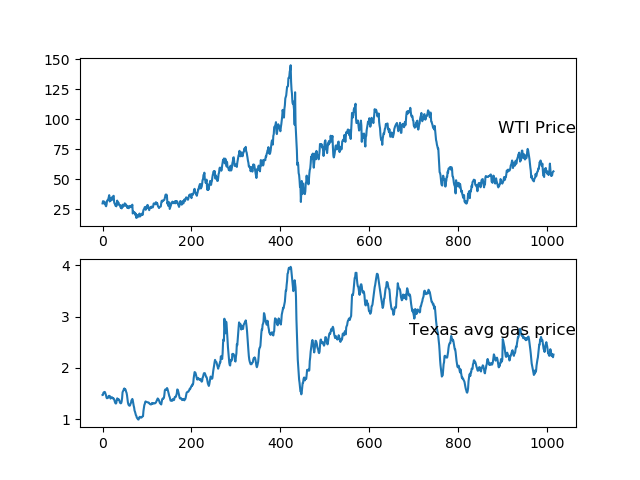
\includegraphics[width=.99\linewidth]{WTI to GasStation relation.png}
\caption{Relation between WTI price and gas station retail prices.}
\label{fig}
\end{figure}

\section{Method and Model}

\subsection{Implementation Reference}

Dr. Jason Brownlee has written about the advantages of Long Short-Term Memory recurrent neural networks over traditional linear methods for forecasting problems with multiple variables/inputs. In his article he shows how to prepare a raw dataset to feed the model, train and use the model to make predictions and rescale the results to original units.[4] 

\subsection{Our Implementation}

Since our data showed that retail prices were dependent on not only current WTI prices, but past ones, and the date/season as well, we implemented our project using a multivariate time series forecast with LSTM recurrent neural networks. Following Dr. Brownlee's example for preparation, the data needed to be framed as a supervised learning problem and input variables needed to be normalized.[4] Once data was prepared, the model was defined, fitted and trained.[4] Normalization was done through MinMaxScaling using sklearn. And to frame our data as supervised learning, we used 12 rows (12 weeks) to forecast the next weeks value. As mentioned at the end of the Data section, our LSTM network implementation took day and month into account, to learn seasons. After all the data pre-processing, our data consisted of 4 variables(Month, Day, WTI price, Texas Avg retail price) times 12 (12 past weeks) and the current weeks avg gas station price, giving us 49 columns and 1003 rows. As for training and testing our model, we used 936 rows for training, testing on the last 67. We tried several different epoch and batch sizes, settling on 10,000 epochs, and a batch size of 150.

\begin{figure}[htbp]
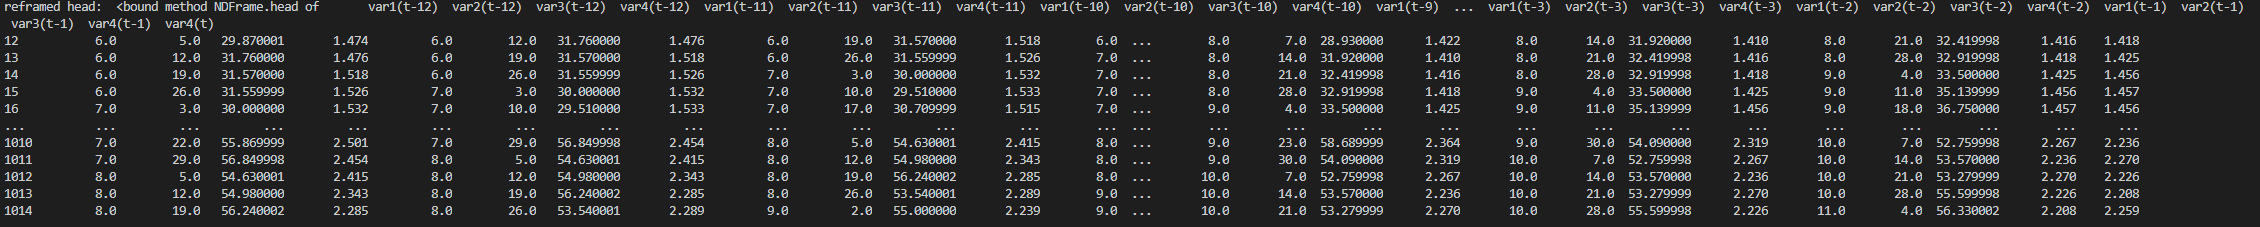
\includegraphics[width=.99\linewidth]{t12tot.png}
\caption{Data after framing}
\label{fig}
\end{figure}

\subsection{Results}

We used root mean square error, rmse, for accuracy measurement. Our rmse on test values ended up at 0.048, so about 5 cents off.

\begin{figure}[htbp]
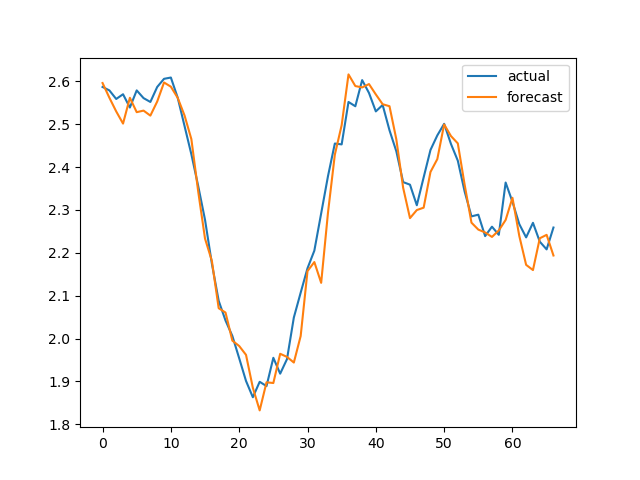
\includegraphics[width=.99\linewidth]{10kActual vs Forecast.png}
\caption{Actual Retail Price vs Model Forecasted Price.}
\label{fig}
\end{figure}

\begin{figure}[htbp]
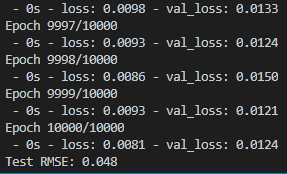
\includegraphics[width=.99\linewidth]{epoch with loss and rmse 10k cropped.png}
\caption{Relation between WTI price and gas station retail prices.}
\label{fig}
\end{figure}

\section{Challenges}

For creating a mobile application that users could use on a regular basis, manually scraping data is not an option. Designing such an application would require, at the very least, weekly updates on gas station prices in all over the US. A backend API with a database would be required. Said database would have to be continually updated with not only WTI barrel prices, but any other crude oil prices that affect retail gas prices in other parts of the country. It may be possible, but we’re not sure on the legalities of continuously gathering data from websites offering up these prices. Also, the hardware requirements to have a server continuously downloading data, and retraining our model as time passed would get costly with electricity alone. We’d need to have many different models (zip code base, or county at least) to be able to accurately predict gas prices where a user is located. In the end, we built a prototype app as a proof of concept for this project.

\section{Hardware}

All training and testing was performed using CPU only. Said CPU was an AMD Ryzen 7 3700x processor with 8 cores and 16 threads.

\section{Conclusion}

Using the data gathered with scrapers and downloaded from the internet, the model tested with above expected accuracy (around 95\%). Though these results are promising, the biggest remaining problem is to implement this project into a working mobile application. In order to gather data from local gas stations, we had to physically visit each one of them and record prices manually since there is no live feed of prices, a method that can hardly be automated. In order to automate this process, a website is needed from which we can gather up-to-date prices frequently and for this to be feasible, we have decided to concentrate on the lower valley area, working with a handful of zip codes and counties.  

Unfortunately, even with such a narrow focus, we have yet to find a reliable website from which we can pull data. If such a website is ever found or created, and the owners allow us to use their data, we can create a database and use it for the application. As for running the server, for this small-scale project, we could absorb costs for a limited time and monitor its success. If the application is popular, there are numerous ways to make it pay for itself, ads being the most obvious. 


\begin{thebibliography}{00}
\bibitem{b1} Kelly Blue Book webpage. [Online]. Available: https://www.kbb.com/most-fuel-efficient-cars/pickup-truck/2019/
\bibitem{b2} U.S. Energy Information Administration webpage. [Online]. Available: \begin{verbatim}https://www.eia.gov/dnav/pet/hist/LeafHandler.ashx?n=pet&s=emm_epmr_pte_stx_dpg&f=w \end{verbatim}
\bibitem{b3} Economic Research Federal Reserve Bank of ST. Louis webpage. [Online]. Available: https://fred.stlouisfed.org/series/DCOILWTICO 
\bibitem{b4} Dr. Jason Brownlee. (2017) Machine Learning Mastery webpage. [Online]. Available: https://machinelearningmastery.com/multivariate-time-series-forecasting-lstms-keras/
\end{thebibliography}
\vspace{12pt}

\end{document}
